\documentclass[12pt,letterpaper]{article}
\usepackage[utf8]{inputenc}
\usepackage{geometry}
\geometry{margin=1in}
\usepackage{graphicx}
\graphicspath{{images/}}
\usepackage{tikz}
\usetikzlibrary{shapes.geometric, arrows}
\usepackage[most]{tcolorbox}
\renewcommand{\baselinestretch}{1.0}

\usepackage{natbib}
\bibliographystyle{plainnat}


\title{\vspace{-3cm}From Narrative Text to Formal Action Language System Descriptions}
\author{Gang Ling}
\date{February 2018}


%\tikzstyle{decision}=[diamond,draw,fill=blue!20,text width=4.5em,text badly centered,node distance=3cm,inner sep=0pt]  
\tikzstyle{io} = [trapezium, trapezium left angle=70, trapezium right angle=110, minimum width=2cm, minimum height=0.75cm, text width=6em, text badly centered, draw=black, fill=blue!20]
\tikzstyle{process1}=[rectangle,draw,fill=green!20,text width=8.5em,text badly centered,rounded corners,minimum height=3em] 
\tikzstyle{process2}=[rectangle,draw,fill=orange!20,text width=8.5em,text badly centered,rounded corners,minimum height=3em] 
\tikzstyle{arrow}=[draw,-latex']  
\tikzstyle{startstop}=[draw,ellipse,fill=red!20,node distance=3cm,minimum height=2.5em]  

\begin{document}
	
	\maketitle
	
	\subsection*{Introduction}
	Computational linguists have long studied various logic forms for capturing essential semantic information carried by narratives. Among these logic forms, discourse representation structure (DRS) form\citep{kampreyle93} is designed to acquire the entities, entities’ property, events, event types, the occurring time of events, and event arguments. In this paper, we describe a system called Text2DRS that takes English narrative as an input and outputs DRS in Neo-Davidsonian style. In this regard, it is similar to Boxer\citep{bos08} which is an open-domain NLP tool for semantic analysis of a text. Boxer also produces a respective DRS of a given narrative. However, Boxer ignores the chronological orders of events in the narrative and misses details in event arguments. Text2DRS captures and provides these missing information. Furthermore, Text2DRS relies on lexical resource VerbNet\citep{KipperPhd05,verbneturl} for annotating the specific relations between relevant entities and events mentioned in the narrative.  
	
	\subsection*{Text2DRS Details}
	Text2DRS is implemented on top of the LTH system\citep{lthurl} and the Standford coreNLP system\citep{manning-EtAl:2014:P14-5}. The LTH is a semantic parser for unrestricted text in English that uses predicates from PropBank\citep{propbank}. The Standford CoreNLP system provides a set of NLP tools including the coreference resolution system. Text2DRS utilizes functions from these two systems for processing given narrative.
	
	\tcbsidebyside[sidebyside adapt=right, blanker, sidebyside gap=1cm, sidebyside align=top seam]{%
		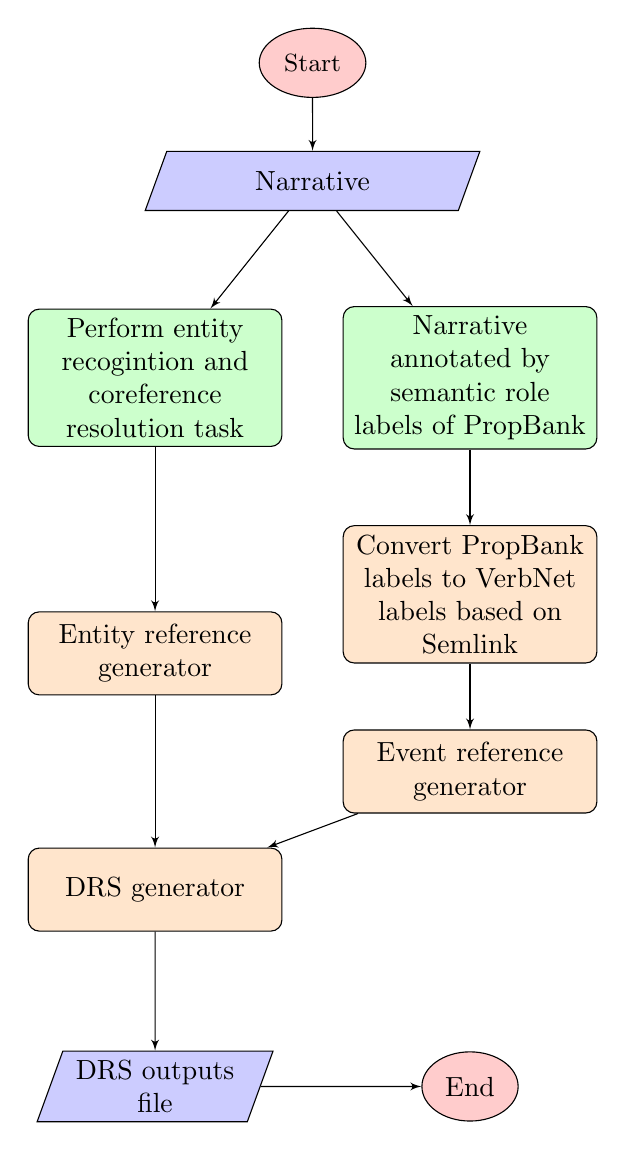
\begin{tikzpicture}[node distance=1.5cm, auto]
		
		\node (start) [startstop] {\small Start};
		\node (in1) [io, below of=start] {Narrative};
		\node (pro1) [process1, below of=in1, xshift=2cm, yshift=-1cm] {Narrative annotated by semantic role labels of PropBank};
		\node (pro2) [process1, below of=in1, xshift=-2cm, yshift=-1cm] {Perform entity recogintion and coreference resolution task};
		\node (pro3) [process2, below of=pro1, yshift=-1.25cm] {Convert PropBank labels to VerbNet labels based on Semlink};
		\node (pro4) [process2, below of=pro2, yshift=-2cm] {Entity reference generator};
		\node (pro5) [process2, below of=pro3, yshift=-0.75cm] {Event reference generator};
		\node (pro6) [process2,below of=pro4, yshift=-1.5cm] {DRS generator};;
		\node (pro7) [io,below of=pro6, yshift=-1cm] {DRS outputs file};
		\node (end) [startstop, right of=pro7,xshift=1cm] {End};
		
		
		\draw[arrow] (start) -- (in1);
		\draw[arrow] (in1) -- (pro1);
		\draw[arrow] (in1) -- (pro2);
		\draw[arrow] (pro1) -- (pro3);
		\draw[arrow] (pro2) -- (pro4);
		\draw[arrow] (pro3) -- (pro5);
		\draw[arrow] (pro4) -- (pro6);
		\draw[arrow] (pro5) -- (pro6);
		\draw[arrow] (pro6) -- (pro7);
		\draw[arrow] (pro7) -- (end);
		
		\end{tikzpicture}%
	}
	{}
    \subsection*{Conclusion}
\bibliography{Text2DRS}
\end{document}